The implementation of Cloud Simplify is designed as an AWS-focused orchestration stack that translates user intent into reproducible infrastructure actions. The implementation objective is not only feature delivery, but operational determinism: identical inputs should result in predictable execution paths, auditable state transitions, and observable outcomes.

\subsection{Implementation Design Principles}
The platform is built around four design principles:
\begin{itemize}
    \item \textbf{Separation of concerns}: user interaction, API orchestration, background execution, and infrastructure provisioning are isolated into distinct layers.
    \item \textbf{Asynchronous execution}: expensive runtime operations are shifted to queue workers to preserve API responsiveness.
    \item \textbf{Explicit state transitions}: deployment statuses are persisted and exposed to prevent hidden execution phases.
    \item \textbf{Security-by-default}: credentials remain encrypted at rest and are only materialized in short-lived worker contexts.
\end{itemize}

\subsection{Technology Stack with References}
Each layer of the system uses a well-established toolchain with explicit technical purpose and documented references, summarized in Table \ref{tab:techstack}.

\begin{table}[h]
\centering
\caption{Technology Stack, Role, and Primary References}
\label{tab:techstack}
\begin{tabular}{|p{2.6cm}|p{2.7cm}|p{4.2cm}|p{2.7cm}|}
\hline
\textbf{Layer} & \textbf{Technology} & \textbf{Role in This Project} & \textbf{Reference} \\ \hline
Frontend & React + Vite & Single-page web interface for credentials, resources, dashboards, and deployments. & \cite{react_docs_2026, vite_docs_2026} \\ \hline
Backend API & FastAPI (Python) & Authenticated REST endpoints for orchestration, billing, and inventory analytics. & \cite{fastapi_docs_2026} \\ \hline
Data Layer & PostgreSQL & Persistent storage for users, credentials, resources, and cost records. & \cite{postgresql_docs_2026} \\ \hline
Async Execution & Celery + Redis & Background task queue for sync and provisioning without blocking API requests. & \cite{celery_docs, redis_docs_2026} \\ \hline
IaC Engine & Terraform & Declarative provisioning workflow (\texttt{init/plan/apply}) for AWS modules. & \cite{hashicorp2024terraform} \\ \hline
Cloud Integration & boto3 + AWS APIs & AWS service access for EC2, S3, VPC, and Cost Explorer synchronization. & \cite{boto3_docs_2026, aws_ec2_api_docs_2026} \\ \hline
Container Runtime & Docker Compose & Reproducible local and server deployment of API, worker, DB, and broker services. & \cite{docker_docs_2026} \\ \hline
\end{tabular}
\end{table}

\subsection{Service Decomposition and Runtime Responsibilities}
The runtime is composed of cooperating services with explicit responsibilities:
\begin{itemize}
    \item \textbf{Frontend}: captures intent, validates form-level constraints, and displays lifecycle updates.
    \item \textbf{FastAPI}: performs authentication checks, request validation, task dispatch, and response normalization.
    \item \textbf{Redis}: acts as broker for asynchronous orchestration tasks.
    \item \textbf{Celery Worker}: executes synchronization and Terraform lifecycle jobs.
    \item \textbf{PostgreSQL}: stores operational records for resources, health, inventory, and cost traces.
    \item \textbf{Terraform Module Layer}: maps abstract request parameters to AWS-native resources.
\end{itemize}

This decomposition allows each component to scale independently and reduces blast radius when one subsystem degrades.

\subsection{Website Screenshot Placeholders}
The following placeholders indicate where project UI screenshots should be inserted in the final manuscript.

\begin{figure}[h]
    \centering
    \includegraphics[width=0.7\linewidth]{Dashboard.png}
    \caption{Cloud Simplify Dashboard Overview}
    \label{fig:placeholder}
\end{figure}


\begin{figure}[h]
    \centering
    \includegraphics[width=0.7\linewidth]{Cloud_Accounts.png}
    \caption{AWS Cloud Account}
    \label{fig:placeholder}
\end{figure}

\begin{figure}[h]
    \centering
    \includegraphics[width=0.75\linewidth]{Credentials.png}
    \caption{AWS Credential Registration Interface}
    \label{fig:placeholder}
\end{figure}


\begin{figure}[h]
    \centering
    \includegraphics[width=0.75\linewidth]{Create_Resource.png}
    \caption{AWS VM/Storage provisioning form with configuration inputs}
    \label{fig:placeholder}
\end{figure}


\begin{figure}[h]
    \centering
    \includegraphics[width=0.75\linewidth]{Deployment.png}
    \caption{Deployment Tracking and Execution Logs}
    \label{fig:placeholder}
\end{figure}


\subsection{Core Execution Workflows}

\subsubsection{Authentication Flow}
The authentication path uses JWT-based authorization, where frontend credentials are validated by the API and a signed token is returned for subsequent calls.

\begin{figure}[h]
\centering
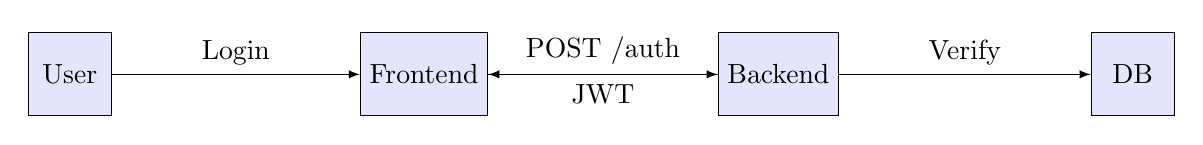
\begin{tikzpicture}[node distance=4.5cm, auto]
    \tikzstyle{actor} = [rectangle, draw, fill=blue!10, minimum width=3em, minimum height=3em]
    \tikzstyle{line} = [draw, -latex]

    \node [actor] (user) {User};
    \node [actor, right of=user] (front) {Frontend};
    \node [actor, right of=front] (back) {Backend};
    \node [actor, right of=back] (db) {DB};

    \draw [line] (user) -- node {Login} (front);
    \draw [line] (front) -- node {POST /auth} (back);
    \draw [line] (back) -- node {Verify} (db);
    \draw [line, dashed] (back) -- node {JWT} (front);
\end{tikzpicture}
\caption{Authentication Sequence}
\label{fig:auth_flow}
\end{figure}

\subsubsection{AWS Provisioning Lifecycle}
Provisioning requests are validated quickly at API layer and then delegated to worker processes for Terraform execution.

\begin{figure}[h]
\centering
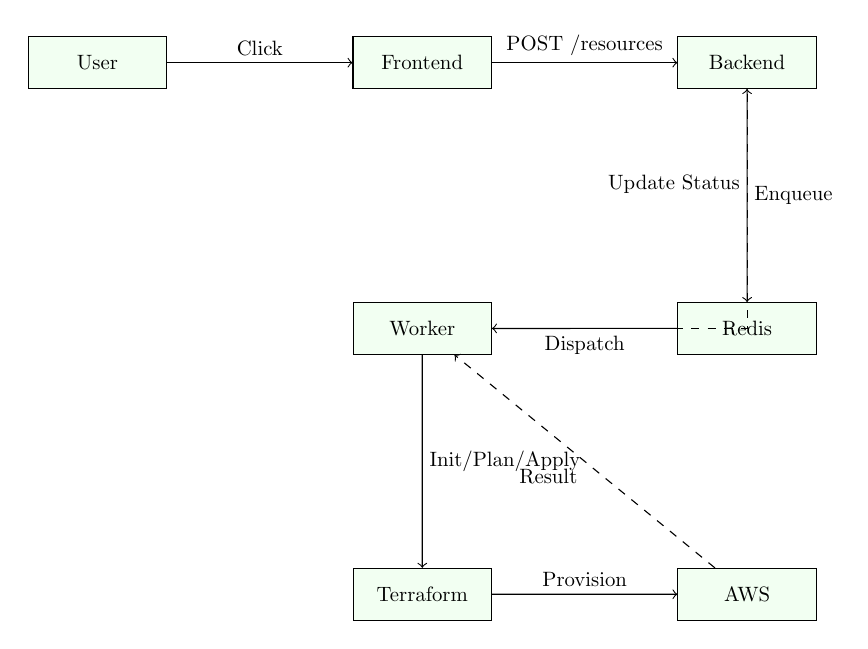
\begin{tikzpicture}[node distance=4.5cm, auto, scale=0.75, every node/.style={scale=0.75}]
    \tikzstyle{comp} = [rectangle, draw, fill=green!5, text width=6em, text centered, minimum height=2.5em]
    \node [comp] (u) {User};
    \node [comp, right of=u, xshift=1cm] (f) {Frontend};
    \node [comp, right of=f, xshift=1cm] (b) {Backend};
    \node [comp, below of=b] (r) {Redis};
    \node [comp, left of=r, xshift=-1cm] (w) {Worker};
    \node [comp, below of=w] (t) {Terraform};
    \node [comp, right of=t, xshift=1cm] (c) {AWS};

    \draw [->] (u) -- node {Click} (f);
    \draw [->] (f) -- node {POST /resources} (b);
    \draw [->] (b) -- node {Enqueue} (r);
    \draw [->] (r) -- node {Dispatch} (w);
    \draw [->] (w) -- node {Init/Plan/Apply} (t);
    \draw [->] (t) -- node {Provision} (c);
    \draw [->, dashed] (c) -- node {Result} (w);
    \draw [->, dashed] (w) -| node[pos=0.8] {Update Status} (b);
\end{tikzpicture}
\caption{AWS Provisioning Lifecycle}
\label{fig:lifecycle}
\end{figure}

\subsection{Code-Level Trace and Layer Coupling}
The execution path from UI action to infrastructure provisioning is traceable across application layers.

\begin{figure}[h]
\centering
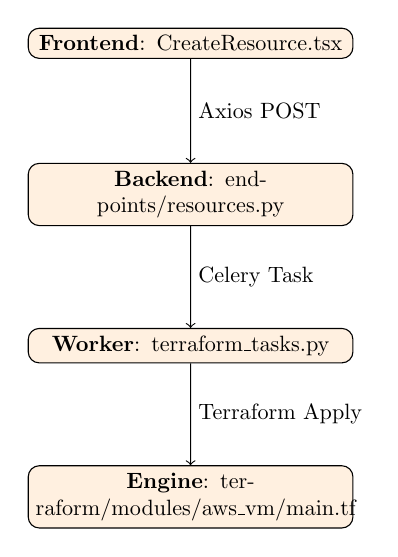
\begin{tikzpicture}[node distance=2.4cm, auto, scale=0.8, every node/.style={scale=0.8}]
    \tikzstyle{layer} = [rectangle, draw, fill=orange!12, text width=14em, text centered, rounded corners]

    \node [layer] (l1) {\textbf{Frontend}: CreateResource.tsx};
    \node [layer, below of=l1] (l2) {\textbf{Backend}: endpoints/resources.py};
    \node [layer, below of=l2] (l3) {\textbf{Worker}: terraform\_tasks.py};
    \node [layer, below of=l3] (l4) {\textbf{Engine}: terraform/modules/aws\_vm/main.tf};

    \draw [->] (l1) -- node {Axios POST} (l2);
    \draw [->] (l2) -- node {Celery Task} (l3);
    \draw [->] (l3) -- node {Terraform Apply} (l4);
\end{tikzpicture}
\caption{Code Trace from UI to AWS Provisioning}
\label{fig:code_trace}
\end{figure}

\subsection{Data Model and Operational Entities}
The platform's persistence layer supports both transactional control and analytical visibility. Key entities include:
\begin{itemize}
    \item \textbf{Cloud credentials}: encrypted provider access records associated with user accounts.
    \item \textbf{Resource inventory}: normalized representation of discovered AWS resources with status and metadata.
    \item \textbf{Provider health}: periodic API connectivity and latency records.
    \item \textbf{Cost data}: service-level spend artifacts used for dashboard and billing summaries.
    \item \textbf{Provisioned resources}: Terraform-managed objects with lifecycle status and execution output.
\end{itemize}

This schema design supports both control-plane actions and retrospective analysis.

\subsection{Security and Credential Lifecycle}
Security is implemented using a zero-trust execution model.
\begin{itemize}
    \item \textbf{Identity Layer}: JWT authentication protects API endpoints and user-specific operations.
    \item \textbf{Credential Security}: AWS access keys are encrypted at application layer and only decrypted inside worker execution scope.
    \item \textbf{Execution Isolation}: Terraform runs in isolated workspaces with ephemeral task context, reducing credential exposure.
    \item \textbf{Surface minimization}: user interfaces never expose raw provider secrets after submission.
\end{itemize}

\subsection{Provisioning Logic and Failure Handling}
The core provisioning routine in \texttt{terraform\_tasks.py} dynamically creates a workspace, injects provider credentials as environment variables, and executes the three-stage Terraform lifecycle: \textit{init}, \textit{plan}, and \textit{apply}. Failure handling is explicit: if initialization, planning, or apply stages fail, resource state is marked accordingly and execution logs are persisted for diagnostics. This behavior is essential for operational transparency in asynchronous systems.

\subsection{Reproducibility Considerations}
Implementation reproducibility is supported through containerized deployment, environment-variable based configuration, deterministic Terraform module selection, and stored execution artifacts. These choices improve comparability across environments and make the paper's reported behavior easier to validate in follow-up studies.
